\documentclass[12pt]{report}

\usepackage[language=english, type=bachelor]{style}
\usepackage{amsmath}
\usepackage{array}
\usepackage{booktabs}
\usepackage{enumitem}
\usepackage{longtable}
\usepackage{fancyhdr}

\pagestyle{fancy}
\lhead{}
\chead{}
\setlength{\headheight}{14.5pt}
\renewcommand{\headrulewidth}{0.2pt}
\renewcommand{\footrulewidth}{0.2pt}

\begin{document}

\specialization{Computer Science}
\title{CitySense Mobile App}
\author{Predescu Mihai Andrei}
\supervisor{Lector Universitar, Dr. Ing. Bara Paul}

\maketitle

\newpage
\pagenumbering{arabic}

\chapter*{Abstract}
\addcontentsline{toc}{chapter}{Abstract}

Urban infrastructure maintenance depends on citizens reporting defects such as potholes, yet many municipal reporting flows still require manual category selection, detailed text input, and repeated submissions for the same issue. These limitations create friction for citizens and noisy datasets for local authorities. This thesis presents \textbf{CitySense}, an Android-first mobile reporting system that reduces that friction by combining smartphone capture, backend object detection, and geospatial deduplication.

The proposed system consists of a Flutter mobile application, a FastAPI backend, a PostgreSQL database extended with PostGIS, and a lightweight web dashboard for administrators. Citizens report a road issue by taking a photograph in the mobile app. The application automatically captures the current GPS coordinates and submits both the image and the location to the backend. A YOLOv8n detector fine-tuned on a pothole dataset classifies the report as a pothole, while the geospatial layer checks whether an open issue of the same type already exists within a configurable radius. When a nearby report is found, the system merges the new submission with the existing ticket and increments its priority through an upvote mechanism instead of inserting a duplicate row.

The contribution of the project is primarily systems-oriented. It demonstrates how mobile development, REST APIs, geospatial querying, and computer vision can be integrated into a single civic technology workflow. In addition to the implementation itself, the thesis documents the design choices behind the data model, the duplicate detection strategy, the Android-first user experience, the detector training process, and the confidence-threshold calibration used before inserting reports into the database. The resulting prototype provides a clear foundation for future work such as multi-class defect detection and municipality-specific deployment.

\tableofcontents

\newpage

\chapter{Introduction}

Maintaining urban infrastructure is a continuous challenge for local authorities. Potholes, damaged road markings, broken public furniture, and illegal dumping all reduce safety and quality of life, yet these issues are often discovered too late or reported through inconvenient channels. Traditional reporting forms usually ask citizens to manually choose a category, describe the problem in text, and specify a location. This introduces friction for citizens and creates inconsistent data for municipalities. The broader problem is therefore not only detection of infrastructure defects, but also the design of a reporting workflow that encourages participation while keeping the resulting data actionable.

This thesis addresses that problem through \textbf{CitySense}, a mobile-first pothole reporting system that combines computer vision, geographic information processing, and cross-platform mobile development. In the proposed workflow, a citizen uses a smartphone to capture a photo of a pothole. The mobile client records the current GPS coordinates and forwards the report to a backend service. The backend then performs two automated steps: it classifies the image as a pothole through a YOLO-based detector \cite{jocher2023ultralytics} and it checks whether a similar open issue already exists nearby by using PostGIS proximity queries \cite{obe2021postgis}. If a nearby report is found, the submission is merged as an additional vote instead of being inserted as a duplicate ticket.

\section{Motivation}

The motivation for the project is both practical and technical. From the practical perspective, citizens often notice infrastructure defects during routine activities such as commuting, walking, or driving, yet many do not report them because the process is slow or unclear. The Federal Highway Administration has documented that collective-information applications can support transportation safety data collection, but their effectiveness depends heavily on ease of use and the quality of the gathered data \cite{fhwa2022collective}. In the context of pothole management, Cheng shows that mobile reporting can improve how defects are tracked and prioritized, especially when citizens are directly involved in the reporting loop \cite{cheng2024potholeprogram}. These observations motivated the search for a more automated reporting pipeline.

The technical motivation comes from the opportunity to combine several modern software engineering domains into a single, cohesive application. Flutter makes it possible to create a mobile interface from one codebase \cite{flutter_docs}. FastAPI provides a compact and expressive way to build Python REST services \cite{fastapi_docs}. YOLO-based detectors are fast enough to support practical image analysis workflows \cite{redmon2016yolo, jocher2023ultralytics}. PostGIS extends relational storage with spatial operators that are essential for duplicate detection based on geographic distance \cite{obe2021postgis}. CitySense brings these technologies together in a real-world civic use case.

\section{Problem Statement}

The problem addressed in this thesis can be stated as follows:

\begin{quote}
How can a civic reporting application reduce manual user input while preventing duplicate pothole tickets and still provide a simple operational view for administrators?
\end{quote}

To answer this question, the system must satisfy several constraints at the same time. The mobile workflow must remain simple enough for non-technical users. The backend must provide a stable API and a clear data model. The detector must expose only the classes that the system truly supports. The database must treat location as a first-class concern rather than an afterthought. Finally, the administrator-facing interface must show a clean and prioritized list of open issues rather than an uncontrolled stream of near-identical reports.

\section{Objectives}

The main objectives of the project are the following:

\begin{enumerate}[label=\arabic*.]
  \item Design and implement an Android-first mobile application that allows citizens to capture pothole reports using a camera-driven workflow.
  \item Build a backend service that accepts image uploads and geographic coordinates through a documented REST API.
  \item Integrate a YOLO-based detector that classifies a report as a pothole and returns a confidence score.
  \item Use PostGIS to merge reports that refer to the same pothole when they are within a configurable spatial radius.
  \item Provide a lightweight administrative dashboard that visualizes reports on top of OpenStreetMap \cite{openstreetmap} and supports status management.
  \item Document the architecture, implementation choices, and evaluation strategy in a complete bachelor thesis.
\end{enumerate}

\section{Contributions}

The contributions of the thesis are primarily engineering-oriented rather than algorithmic. The detector itself is not presented as a novel computer vision architecture. Instead, the project contributes:

\begin{itemize}
  \item an end-to-end software prototype that connects mobile capture, REST communication, object detection, and geospatial duplicate handling;
  \item a report data model that explicitly separates issue type, geographic position, status, and priority;
  \item a duplicate-merging workflow that turns repeated reports into upvotes instead of redundant database rows;
  \item an operational dashboard that links geographic context with report status and upvote counts;
  \item a reproducible monorepo structure that keeps implementation and thesis artifacts synchronized.
\end{itemize}

\section{Thesis Structure}

Chapter 2 introduces the technologies that underpin the application, with emphasis on Flutter, FastAPI, YOLO-based detection, and PostGIS. Chapter 3 reviews related work in both civic issue reporting and road-damage detection. Chapter 4 presents the architecture and implementation of CitySense. Chapter 5 evaluates the resulting system through functional scenarios and discusses detector readiness and current limitations. Chapter 6 concludes the thesis and outlines directions for future work.

\part{Theoretical Part}
\chapter{Theoretical Background}

CitySense combines mobile computing, backend web services, computer vision, and geographic information systems. This chapter summarizes the concepts that are most relevant to the implementation.

\section{Cross-Platform Mobile Development with Flutter}

Flutter is a cross-platform UI toolkit that enables the development of mobile applications from a single Dart codebase \cite{flutter_docs}. Instead of relying on a bridge to native widgets, Flutter renders its own widget tree, which makes the visual layer consistent across platforms. For a project like CitySense, this is useful because the interaction is strongly guided by a small set of reusable screens: a camera-driven reporting view, a map view, and status feedback components.

Another relevant feature is Flutter's plugin ecosystem. Access to the device camera and location sensors is exposed through packages that wrap platform-specific behavior behind a single interface. This makes it possible to build an Android-first prototype without writing a separate Kotlin application from scratch, while still preserving the possibility of extending the same client to iOS later.

\section{Python APIs with FastAPI}

FastAPI is a Python web framework designed around asynchronous request handling, automatic request validation, and concise API definitions \cite{fastapi_docs}. It is well suited to CitySense because the backend requirements are clear and structured: accept multipart form uploads, validate coordinates, expose JSON report data, and render an administrative HTML page.

The framework also integrates naturally with Pydantic-based schemas, which is helpful when the same data model must be used consistently across multiple endpoints. In CitySense, the backend exposes health, report submission, report listing, and status update endpoints. Each endpoint benefits from explicit request and response schemas because the mobile client and the dashboard depend on predictable field names and types.

\section{Object Detection and YOLO-Based Inference}

Object detection differs from image classification in that it must identify both the class of an object and its approximate position in the image. The original YOLO formulation reframed detection as a single-stage regression problem, allowing the network to predict classes and bounding boxes in one pass \cite{redmon2016yolo}. This approach made it possible to trade some complexity in favor of real-time or near-real-time inference.

The implementation used in this project is based on Ultralytics YOLO \cite{jocher2023ultralytics}. In practical terms, the detector receives an image and returns one or more bounding boxes with associated classes and confidence scores. For CitySense, the backend accepts only pothole-related labels as valid output. This normalization step is important because a general-purpose detector may return classes that are outside the scope of the application. The system therefore treats the detector not as a free-form classifier but as a bounded service with a clearly defined output contract.

\section{Spatial Data and PostGIS}

PostgreSQL is a relational database system with strong support for transactional integrity, indexing, and structured queries \cite{postgres_docs}. PostGIS extends PostgreSQL with spatial types and spatial functions, which makes it possible to store locations as geographic objects and query them by distance \cite{obe2021postgis}. This is essential for CitySense because duplicate detection is fundamentally a spatial problem.

The core function used in the implementation is \texttt{ST\_DWithin}. Given two geographic points and a distance threshold, this function checks whether the points are within that threshold. By storing each report as a point geometry and using a fixed radius, the backend can decide whether a new pothole report should become a fresh ticket or an upvote on an existing one. This is more robust than comparing latitude and longitude directly because it treats geographic distance as the real business rule.

\section{Map Rendering with OpenStreetMap and Leaflet}

An administrator-facing map is useful only if it provides geographic context and remains easy to interpret. CitySense uses OpenStreetMap tiles as the geographic base layer \cite{openstreetmap}. The web dashboard uses Leaflet for browser-based map rendering \cite{leaflet_docs}, while the mobile client uses Flutter map rendering components built on the same OpenStreetMap tile model. The shared map foundation ensures that administrators and citizens interpret issue locations in a consistent geographic frame.

\section{Summary}

The theoretical foundation of CitySense can therefore be summarized as follows: Flutter provides the mobile interaction layer, FastAPI structures the HTTP API, YOLO enables pothole-oriented image analysis, and PostGIS supplies the spatial operators required for duplicate merging. The implementation chapter builds directly on these concepts.

\chapter{Related Work}

\section{Civic Reporting Platforms}

Digital civic reporting is not a new idea, but existing platforms often focus on ticket intake rather than automated interpretation. The Federal Highway Administration discusses several collective-information applications, including systems such as Street Bump, that attempt to collect road-condition signals directly from citizens or drivers \cite{fhwa2022collective}. These platforms show that citizen participation can be valuable, but they also reveal a recurring trade-off: a richer submission form can improve report quality, while a shorter form increases the likelihood that users will report an issue at all.

This trade-off is important for CitySense. Rather than asking the user to manually categorize the issue, the project aims to remove that step and let the backend infer the pothole label from the image. In this sense, CitySense belongs to the same family of civic tools as existing reporting platforms, but it shifts part of the reporting burden from the user to the software stack.

\section{Pothole Management Systems}

Cheng proposes a prototype pothole management program that connects reporting, tracking, and maintenance workflows in a single system \cite{cheng2024potholeprogram}. That work is closely related to the motivation of this thesis because it frames pothole reporting as part of a larger management process rather than as an isolated mobile feature. The report emphasizes that citizen participation, simplified submission, and clear operational handling are all necessary for a useful pothole workflow.

CitySense follows a similar systems perspective, but it differentiates itself in two ways. First, it introduces a vision-based categorization step into the report lifecycle. Second, it uses spatial duplicate merging to reduce database clutter caused by repeated reports from the same location. These choices are intended to support the same operational goal with a stronger automation emphasis.

\section{Road Damage Detection Research}

Road damage detection has become an active research topic in computer vision. Arya et al.\ review state-of-the-art solutions and summarize the challenges of detecting cracks, potholes, and related road defects across varied image conditions \cite{arya2022rdd2022}. A central contribution of this line of work is the Road Damage Detection dataset family, especially RDD2022, which provides a public benchmark across multiple countries and road conditions \cite{arya2022rdd2022}. Public datasets of this type are important because they make it easier to compare models and train defect detectors that generalize beyond a single city or camera setup.

The CitySense project does not attempt to introduce a novel detector architecture. Instead, it adopts the practical position that a modern YOLO-based detector can be integrated into a civic workflow if the system carefully restricts the supported label space and clearly defines the scope of the application. This makes the project closer to applied engineering than pure machine learning research, while still benefiting from the methodological progress of recent detection literature.

\section{Positioning of CitySense}

The closest related systems therefore come from two directions:

\begin{itemize}
  \item civic technology applications that make it easier for citizens to submit and track public-works issues;
  \item computer vision systems that detect road damage from images.
\end{itemize}

CitySense occupies the intersection of these two directions. It is not merely a reporting form with a map, and it is not merely a detector benchmark. Its purpose is to connect image-based pothole recognition with a practical reporting pipeline that includes mobile capture, geospatial duplicate handling, and an administrative view of active issues. This combined focus defines the main niche of the project.

\part{Practical Part}
\chapter{System Design and Implementation}

\section{Architectural Overview}

CitySense is structured as a three-layer system:

\begin{enumerate}[label=\arabic*.]
  \item a Flutter mobile client used by citizens to capture and submit pothole reports;
  \item a FastAPI backend responsible for validation, detection, persistence, and duplicate handling;
  \item a lightweight web dashboard that visualizes active reports and supports status management.
\end{enumerate}

The architectural goal is to keep the mobile workflow small and intuitive while delegating processing-heavy tasks to the backend. Image capture, permission handling, and map viewing remain on the client. Detection, spatial queries, and persistence remain on the server. This separation also keeps the core business logic centralized in one place, which simplifies both testing and thesis documentation.

\section{Mobile Application}

The mobile client is implemented in Flutter. The application is Android-first in the current version, but the codebase is organized so that API communication, location retrieval, and screen logic are separated into reusable services. The mobile interface contains two principal screens:

\begin{itemize}
  \item a \textbf{Report} screen that captures the image, fetches the current GPS location, submits the report, and displays submission feedback;
  \item a \textbf{Map} screen that displays open reports as markers and allows the user to inspect report metadata.
\end{itemize}

This structure is visible in the application interface shown in Figure~\ref{fig:app_interface}. The screen is intentionally simple because the main design objective is to minimize user friction. Instead of collecting a textual description from the user, the application sends the image and coordinates to the backend and displays the result returned by the detector.

\begin{figure}[htbp]
    \centering
    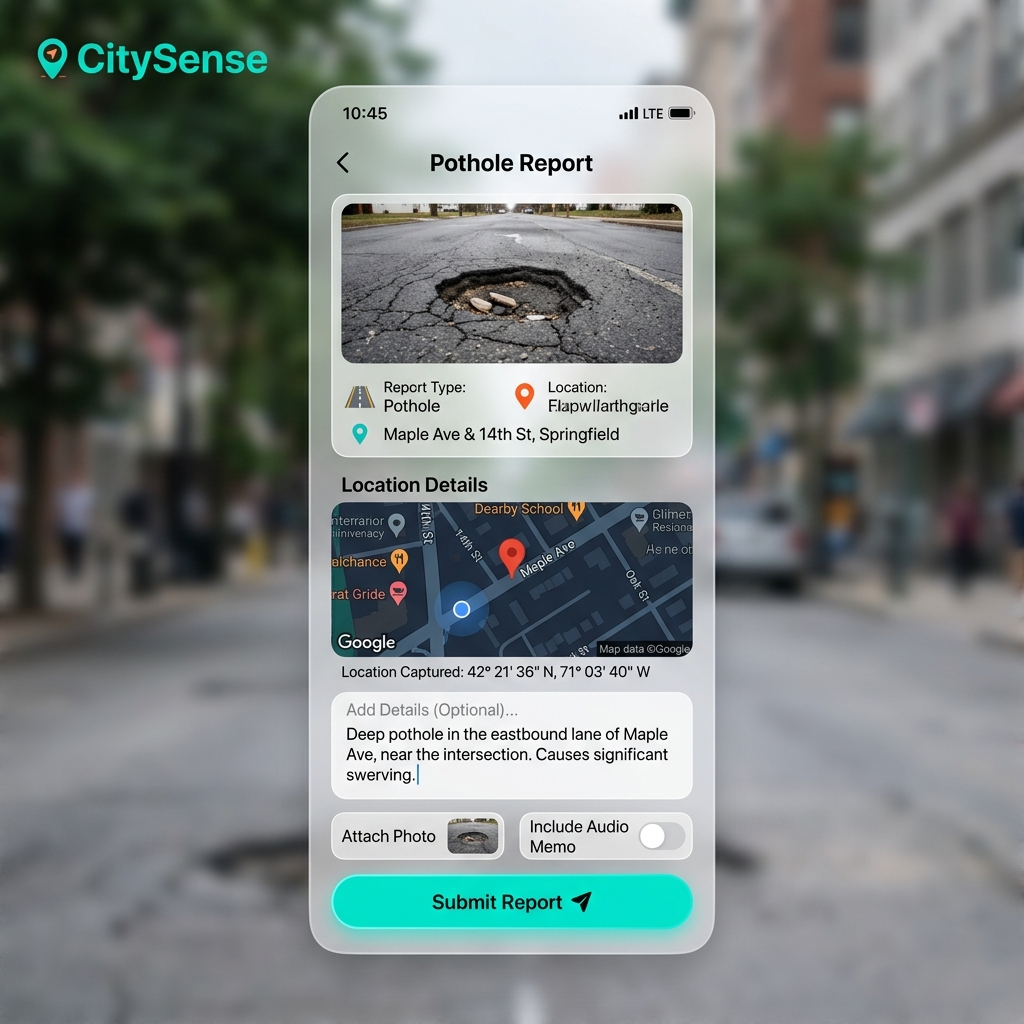
\includegraphics[width=0.45\textwidth]{figures/app_interface_pothole_1775200631079.png}
    \caption{CitySense mobile application interface for photo-based pothole reporting.}
    \label{fig:app_interface}
\end{figure}

\section{Backend Service}

The backend is implemented in Python with FastAPI. It exposes a small REST interface that matches the needs of the mobile client and the admin dashboard. The current API surface is summarized in Table~\ref{tab:api_endpoints}.

\begin{table}[htbp]
\centering
\begin{tabular}{>{\raggedright\arraybackslash}p{0.28\linewidth} >{\raggedright\arraybackslash}p{0.62\linewidth}}
\toprule
\textbf{Endpoint} & \textbf{Purpose} \\
\midrule
\texttt{GET /api/v1/health} & Returns runtime information such as detector mode, upload directory, and duplicate radius. \\
\texttt{POST /api/v1/reports} & Accepts a pothole image and geographic coordinates, runs detection, and either creates or merges a report. \\
\texttt{GET /api/v1/reports} & Returns report data for the mobile map and the admin dashboard. \\
\texttt{PATCH /api/v1/reports/\{id\}/status} & Updates a report from \texttt{OPEN} to \texttt{RESOLVED}. \\
\bottomrule
\end{tabular}
\caption{Public backend endpoints used by CitySense.}
\label{tab:api_endpoints}
\end{table}

The backend uses SQLAlchemy models to persist reports in PostgreSQL. Each report stores the issue type, detector confidence, latitude, longitude, geographic point, image path, status, upvote count, and timestamps. The system currently focuses on the \texttt{pothole} issue type because that keeps the label space explicit and consistent with the intended detector workflow.

\section{Duplicate Detection with PostGIS}

One of the most important implementation details is the duplicate merge strategy. A new report is not automatically inserted as a new row. Instead, the backend constructs a geographic point from the incoming latitude and longitude and compares it against open reports of the same issue type. The comparison is performed with \texttt{ST\_DWithin}, using a 10 meter threshold.

If a matching open report already exists, the new submission increments the upvote counter of the existing record. If no match is found, the backend creates a new report. This design keeps the map readable and makes the administrative view more useful, because repeat submissions become a signal of urgency rather than database noise.

\section{Detection Pipeline}

The detector layer is implemented as a dedicated backend service. In the intended thesis configuration, the backend loads a trained pothole checkpoint and accepts only pothole-like labels from the detector output. The implementation also includes a clearly marked \texttt{demo} detector mode that returns deterministic pothole responses for UI smoke testing when a trained checkpoint is not yet present. This decision keeps the rest of the stack testable without pretending that a generic detector is sufficient for pothole recognition.

Figure~\ref{fig:yolo_detection} shows a sample detection-style output used to illustrate the intended visual feedback of the YOLO pipeline. The repository also includes scripts for fine-tuning and evaluation so that a dedicated pothole checkpoint can be produced from an RDD2022-style dataset.

\begin{figure}[htbp]
    \centering
    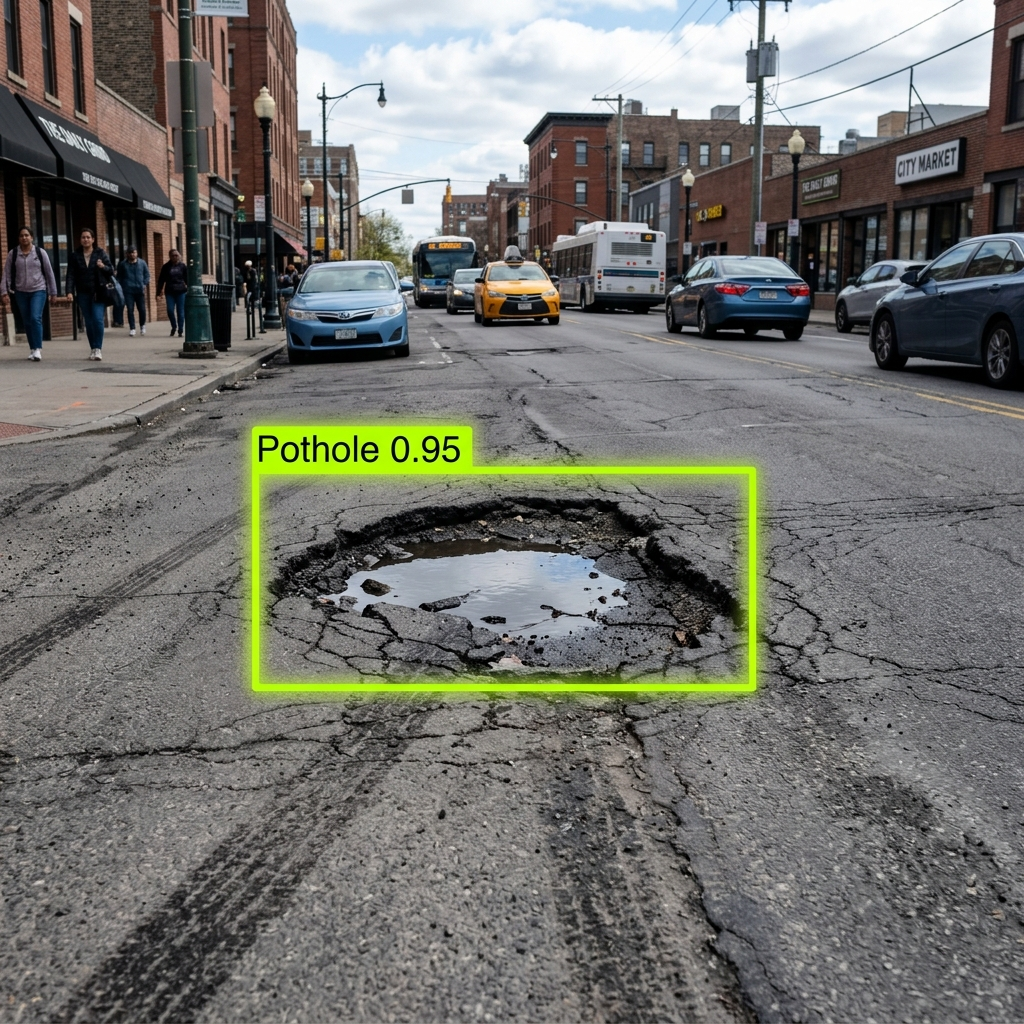
\includegraphics[width=0.78\textwidth]{figures/yolo_detection_demo_1775200664858.png}
    \caption{Illustrative detector output for the CitySense pothole-recognition pipeline.}
    \label{fig:yolo_detection}
\end{figure}

\section{Administrative Dashboard}

The administrator-facing interface is a lightweight web page built around Leaflet and OpenStreetMap tiles. It is intentionally separate from the mobile client because the administrative role requires a different view of the data: status filters, marker clustering by proximity, direct access to upvote counts, and the ability to mark a report as resolved.

Figure~\ref{fig:admin_dashboard} presents the dashboard concept used in the project. The current implementation shows report cards, a geographic map layer, report metadata, and a resolve action. This is enough to support the demonstration scenario of the thesis without overextending the scope into a full municipal operations platform.

\begin{figure}[htbp]
    \centering
    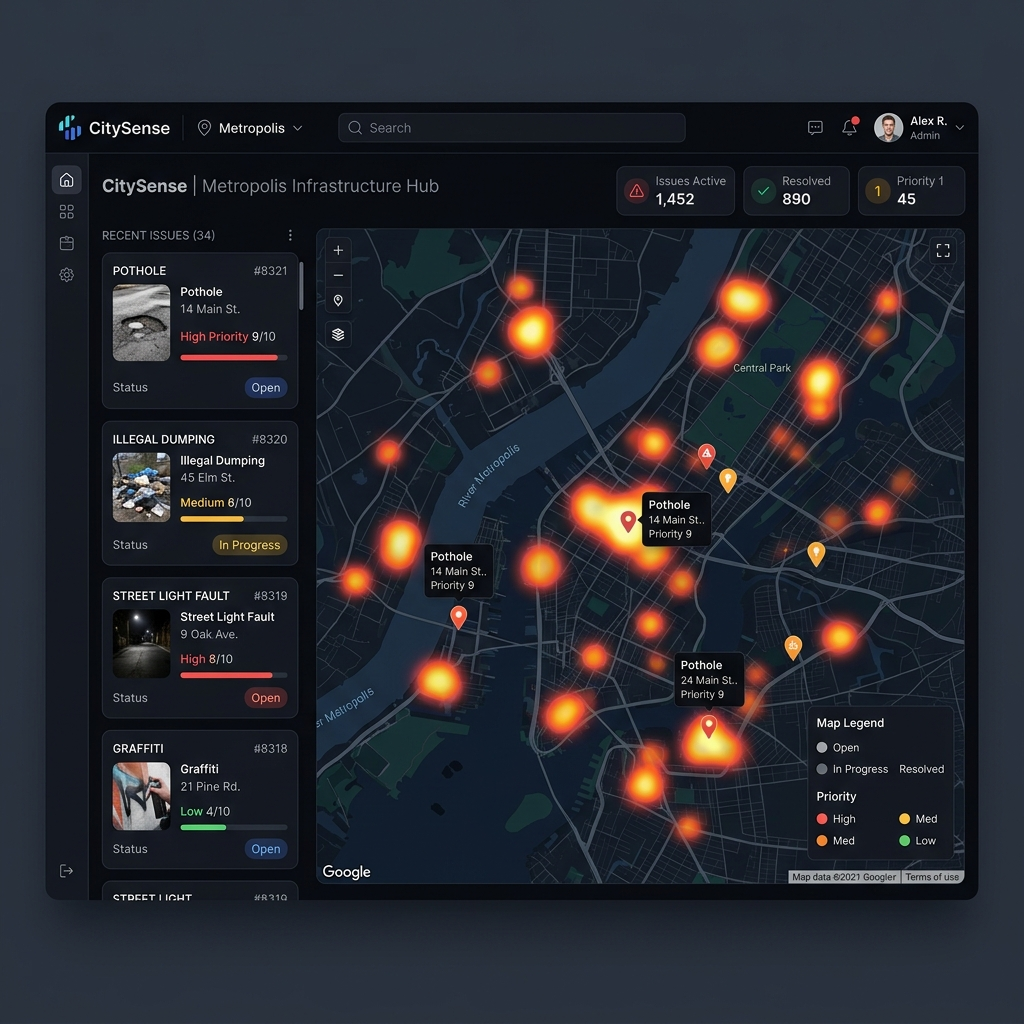
\includegraphics[width=0.85\textwidth]{figures/admin_dashboard_map_1775200648148.png}
    \caption{Administrative dashboard for viewing and resolving reported potholes.}
    \label{fig:admin_dashboard}
\end{figure}

\section{Monorepo Organization}

The final implementation is maintained as a monorepo with three main directories: backend, mobile client, and thesis source. This organization supports reproducibility in two ways. First, it keeps documentation synchronized with code evolution. Second, it makes setup instructions more coherent because the API, the app, and the thesis all live in one repository and can be versioned together.

\chapter{Experimental Evaluation}

\section{Evaluation Strategy}

The evaluation of CitySense focuses on end-to-end software behavior rather than on claiming a new state-of-the-art detector. This choice follows directly from the scope of the project: the main contribution is the integration of mobile reporting, backend processing, and spatial duplicate handling into a single workflow. Therefore, the evaluation emphasizes functional scenarios, qualitative detector readiness, and system limitations.

\section{Functional Scenarios}

Table~\ref{tab:functional_tests} summarizes the main functional scenarios used to evaluate the implementation.

\begin{table}[htbp]
\centering
\begin{tabular}{>{\raggedright\arraybackslash}p{0.28\linewidth} >{\raggedright\arraybackslash}p{0.28\linewidth} >{\raggedright\arraybackslash}p{0.34\linewidth}}
\toprule
\textbf{Scenario} & \textbf{Expected Result} & \textbf{Observed Outcome} \\
\midrule
Health endpoint request & Backend reports runtime configuration & Endpoint returns detector mode, model path, upload directory, and duplicate radius. \\
New pothole report & New database record is created & Implemented through \texttt{POST /api/v1/reports}. \\
Nearby repeat report & Existing ticket is merged and upvotes increase & Implemented through PostGIS \texttt{ST\_DWithin} duplicate checking. \\
Open reports map view & User sees active tickets on a map & Implemented on both the mobile map screen and the admin dashboard. \\
Status update & Administrator marks an issue as resolved & Implemented through \texttt{PATCH /api/v1/reports/\{id\}/status}. \\
UI smoke test without model & Client and backend remain demonstrable & Supported by the explicit backend demo detector mode. \\
\bottomrule
\end{tabular}
\caption{Functional scenarios used to evaluate the CitySense workflow.}
\label{tab:functional_tests}
\end{table}

These scenarios validate the main user journey. A citizen can submit a report, the backend can decide whether to create or merge it, and an administrator can inspect and resolve the resulting issue. This establishes that the software architecture is coherent even before large-scale field deployment.

\section{Detector Readiness}

The computer vision layer is evaluated in a pragmatic manner. The repository includes the infrastructure required to fine-tune a pothole detector on an RDD2022-style dataset \cite{arya2022rdd2022}, as well as a batch evaluation utility for local image folders. The backend also enforces an output contract: only pothole-compatible labels are accepted as valid application results.

At the same time, this thesis does not claim a benchmark-grade quantitative result such as mean average precision on a published test split. A fully reproducible detector benchmark requires a dedicated checkpoint, a stable training environment, and a controlled evaluation dataset. Those steps are prepared in the implementation, but they should be treated as follow-up work rather than as completed experimental evidence. The present document therefore limits itself to qualitative detector integration and to the software behavior that depends on that integration.

\section{Qualitative Observations}

From a software engineering perspective, several observations emerged during implementation:

\begin{itemize}
  \item the mobile workflow benefits significantly from removing manual category selection;
  \item duplicate merging improves the clarity of the map view because repeated reports accumulate as upvotes rather than as overlapping markers;
  \item the administrative dashboard becomes more actionable when status and geographic context are shown together;
  \item separating detector mode from the rest of the backend logic makes the system easier to test without conflating smoke tests with real model evaluation.
\end{itemize}

These observations support the main thesis argument: the value of CitySense comes from the combination of automation and geospatial prioritization, not from any one component in isolation.

\section{Current Limitations}

The current version of CitySense has several limitations that are important to document explicitly:

\begin{enumerate}[label=\arabic*.]
  \item The implementation is pothole-first and does not yet support a broader civic issue taxonomy.
  \item No municipality-specific authentication or work-order integration is included.
  \item Quantitative detector benchmarking is prepared but not yet finalized inside this local environment.
  \item The mobile client is optimized for Android-first demonstration rather than full production deployment across app stores.
\end{enumerate}

These limitations do not invalidate the prototype, but they define the boundary between the implemented system and the broader product vision.

\chapter{Conclusions and Future Work}
\label{conclusions}

This thesis presented CitySense, an Android-first civic reporting platform designed to simplify pothole reporting through mobile capture, offline report storage, backend automation, and geospatial duplicate handling. The final system combines a Flutter mobile application, a local phone-side report queue, a FastAPI backend, a PostgreSQL/PostGIS data layer, and a web dashboard for operational review. Instead of treating each report as an isolated ticket, the system aggregates nearby reports into a single issue with an increasing upvote count. This makes the resulting data more useful for prioritization and more readable on a map.

The work demonstrates that a practical civic reporting pipeline can be built by integrating established technologies rather than inventing a new algorithm from scratch. Flutter supports a simple citizen workflow, SQLite keeps captured reports safe until synchronization, FastAPI and SQLAlchemy provide a clear service boundary, PostGIS supplies the spatial reasoning needed for duplicate merging, and a YOLO-based detector enables automation of the issue classification step. Together, these parts form a coherent software prototype with a clear civic reporting purpose.

At the same time, the project remains intentionally scoped. The system focuses on potholes rather than on a wide taxonomy of municipal issues. A YOLOv8n detector was fine-tuned on a pothole dataset, integrated into the backend as \texttt{pothole\_yolov8n.pt}, evaluated on validation and test splits, and configured with an application confidence threshold of 0.65 after calibration and field testing. This boundary is important because it keeps the written document aligned with the implemented evidence: CitySense is a working pothole-first prototype, not yet a general urban-damage detection platform.

\section{Future Work}

Several future directions follow naturally from the current version. A next version could collect and annotate additional classes such as trash piles, damaged signs, and damaged pole-mounted trash bins, then retrain the detector as a multi-class YOLO model and update the backend label mapping accordingly. It could also add user accounts, municipal roles, and notification workflows. Another useful extension would be to improve offline synchronization with background scheduling and clearer conflict-resolution tools, connect the dashboard to maintenance scheduling or work-order systems, and improve map analytics through clustering, heatmaps, and historical trends.

In summary, CitySense should be understood as a strong prototype and a foundation for subsequent development. Its main accomplishment is not only that it detects or stores potholes, but that it demonstrates a complete reporting loop in which image capture, location, geospatial reasoning, and administrative review are treated as parts of one system.


\bibliography{references}

\end{document}
